\documentclass[border=6pt]{standalone}
\usepackage{tikz}
\usetikzlibrary{arrows.meta,positioning,fit,calc}
\definecolor{fg}{HTML}{DBC9A8}
\definecolor{fgbody}{HTML}{C4A882}
\definecolor{stroke}{HTML}{C4963C}
\definecolor{surf}{HTML}{22222B}
\definecolor{surfemph}{HTML}{2A2820}
\definecolor{surfact}{HTML}{2E2020}
\definecolor{bdim}{HTML}{9A7F62}
\definecolor{bemph}{HTML}{D4A849}
\definecolor{bact}{HTML}{FF5C5C}
\begin{document}
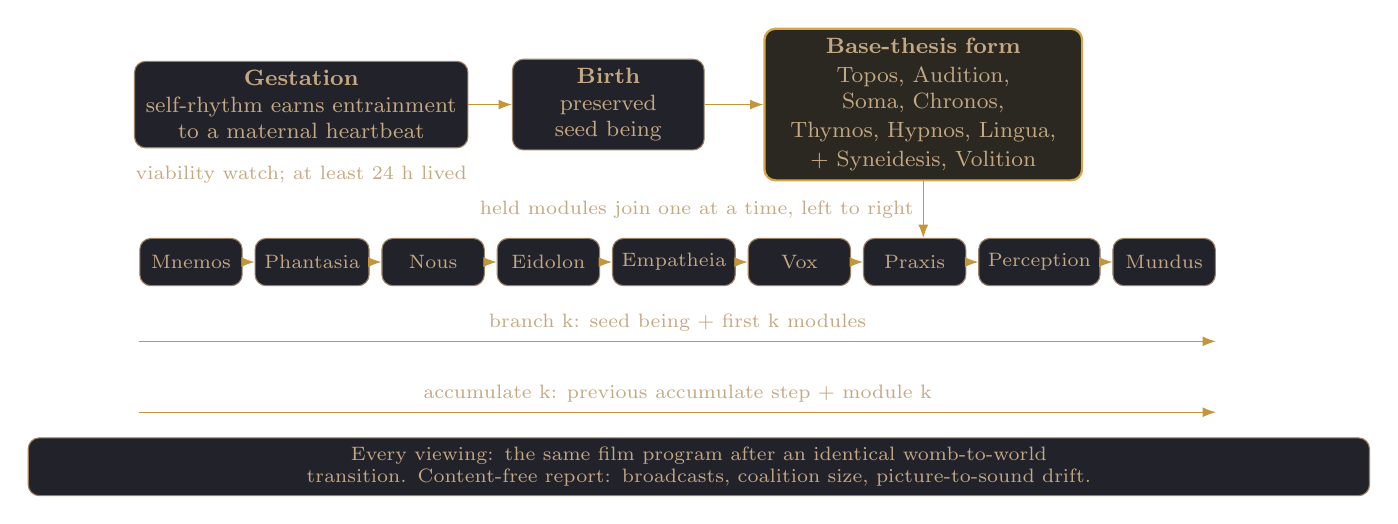
\begin{tikzpicture}[
  font=\footnotesize,>=Latex,
  every node/.append style={text=fgbody, execute at begin node={\hyphenpenalty=10000\exhyphenpenalty=10000}},
  mod/.style={draw=bdim, rounded corners, fill=surf, align=center, font=\footnotesize},
  work/.style={draw=bemph, thick, rounded corners, fill=surfemph, align=center},
  lbl/.style={font=\footnotesize, text=fgbody, align=center},
  held/.style={mod, minimum width=13mm, minimum height=6mm, font=\scriptsize},
]

% Stage 1
\node[mod, text width=40mm] (stage1) at (0,2)
  {\textbf{Gestation}\\self-rhythm earns entrainment\\to a maternal heartbeat};
\node[lbl, font=\scriptsize, below=1mm of stage1]
  {viability watch; at least 24 h lived};

% Stage 2
\node[mod, text width=22mm] (stage2) at (3.9,2)
  {\textbf{Birth}\\preserved seed being};
\draw[->, draw=stroke] (stage1.east) -- (stage2.west);

% Stage 3
\node[work, text width=38mm] (stage3) at (7.9,2)
  {\textbf{Base-thesis form}\\[1pt]
   Topos, Audition, Soma, Chronos,\\[1pt]
   Thymos, Hypnos, Lingua,\\[1pt]
   + Syneidesis, Volition};
\draw[->, draw=stroke] (stage2.east) -- (stage3.west);

% Held modules
\node[held] (m1) at (-1.4,0) {Mnemos};
\node[held, right=1.5mm of m1] (m2) {Phantasia};
\node[held, right=1.5mm of m2] (m3) {Nous};
\node[held, right=1.5mm of m3] (m4) {Eidolon};
\node[held, right=1.5mm of m4] (m5) {Empatheia};
\node[held, right=1.5mm of m5] (m6) {Vox};
\node[held, right=1.5mm of m6] (m7) {Praxis};
\node[held, right=1.5mm of m7] (m8) {Perception};
\node[held, right=1.5mm of m8] (m9) {Mundus};

\draw[->, draw=stroke] (stage3.south) -- (stage3.south |- m1.north) node[midway, left, font=\scriptsize] {held modules join one at a time, left to right};

\foreach \i/\j in {1/2,2/3,3/4,4/5,5/6,6/7,7/8,8/9}{
  \draw[->, draw=stroke] (m\i.east) -- (m\j.west);
}

% Recurrence arrows
\draw[->, draw=stroke, thin]
  ($(m1.south west)+(0,-0.7)$) -- ($(m9.south east)+(0,-0.7)$)
  node[pos=0.5, above, font=\scriptsize] {branch k: seed being + first k modules};
\draw[->, draw=stroke, thin]
  ($(m1.south west)+(0,-1.6)$) -- ($(m9.south east)+(0,-1.6)$)
  node[pos=0.5, above, font=\scriptsize] {accumulate k: previous accumulate step + module k};

% Footer
\node[mod, text width=168mm, font=\scriptsize] at (5.05,-2.6)
  {Every viewing: the same film program after an identical womb-to-world transition.
   Content-free report: broadcasts, coalition size, picture-to-sound drift.};

\end{tikzpicture}
\end{document}
